%!TEX root = ../Pflichtenheft.tex

\chapter{Benutzeroberfläche}
\label{chap:ui}

\section{Haupseite und Buchung}

Die Startseite der Anwendung ist in \ref{fig:startseite} dargestellt.
Auf dieser haben NutzerInnen die Möglichkeit, dem Raum zu buchen oder auf andere Ansichten zu wechseln.
Sollten NuterInnen eine Buchung vornehmen wollen, so klicken diese in den gewünschten Zeitraum
und es wird der Dialog in \ref{fig:buchung} dargestellt.
Hier können NutzerInnen die gewünschte Zeit und den Raum auswählen.
Tätigen NutzerInnen eine Buchung, so werden diese aufgefordert, sich anzumelden.
Der hierzu gehörige Dialog ist in \ref{fig:login} dargestellt.
Alternativ ist dieser Dialog auch über den Anmeldungsbutton, der in Abbildung \ref{fig:startseite} zu sehen ist, erreichbar.
Der Banner in allen Ansichten zeigt den aktuellen Raumstatus an.
Insbesondere wird dadurch die Priorität der aktuellen Buchung mithilfe der Farbe des Banners angezeigt.
Sind NutzerInnen eingeloggt und belegen den Raum,
so wird ihnen die in Abbildung \ref{fig:checkout} dargestellte Ansicht angezeigt.
Hier können NutzerInnen den Raum wieder über den Quick-Checkout Button freigeben.

\begin{figure}[ht]
    \centering
    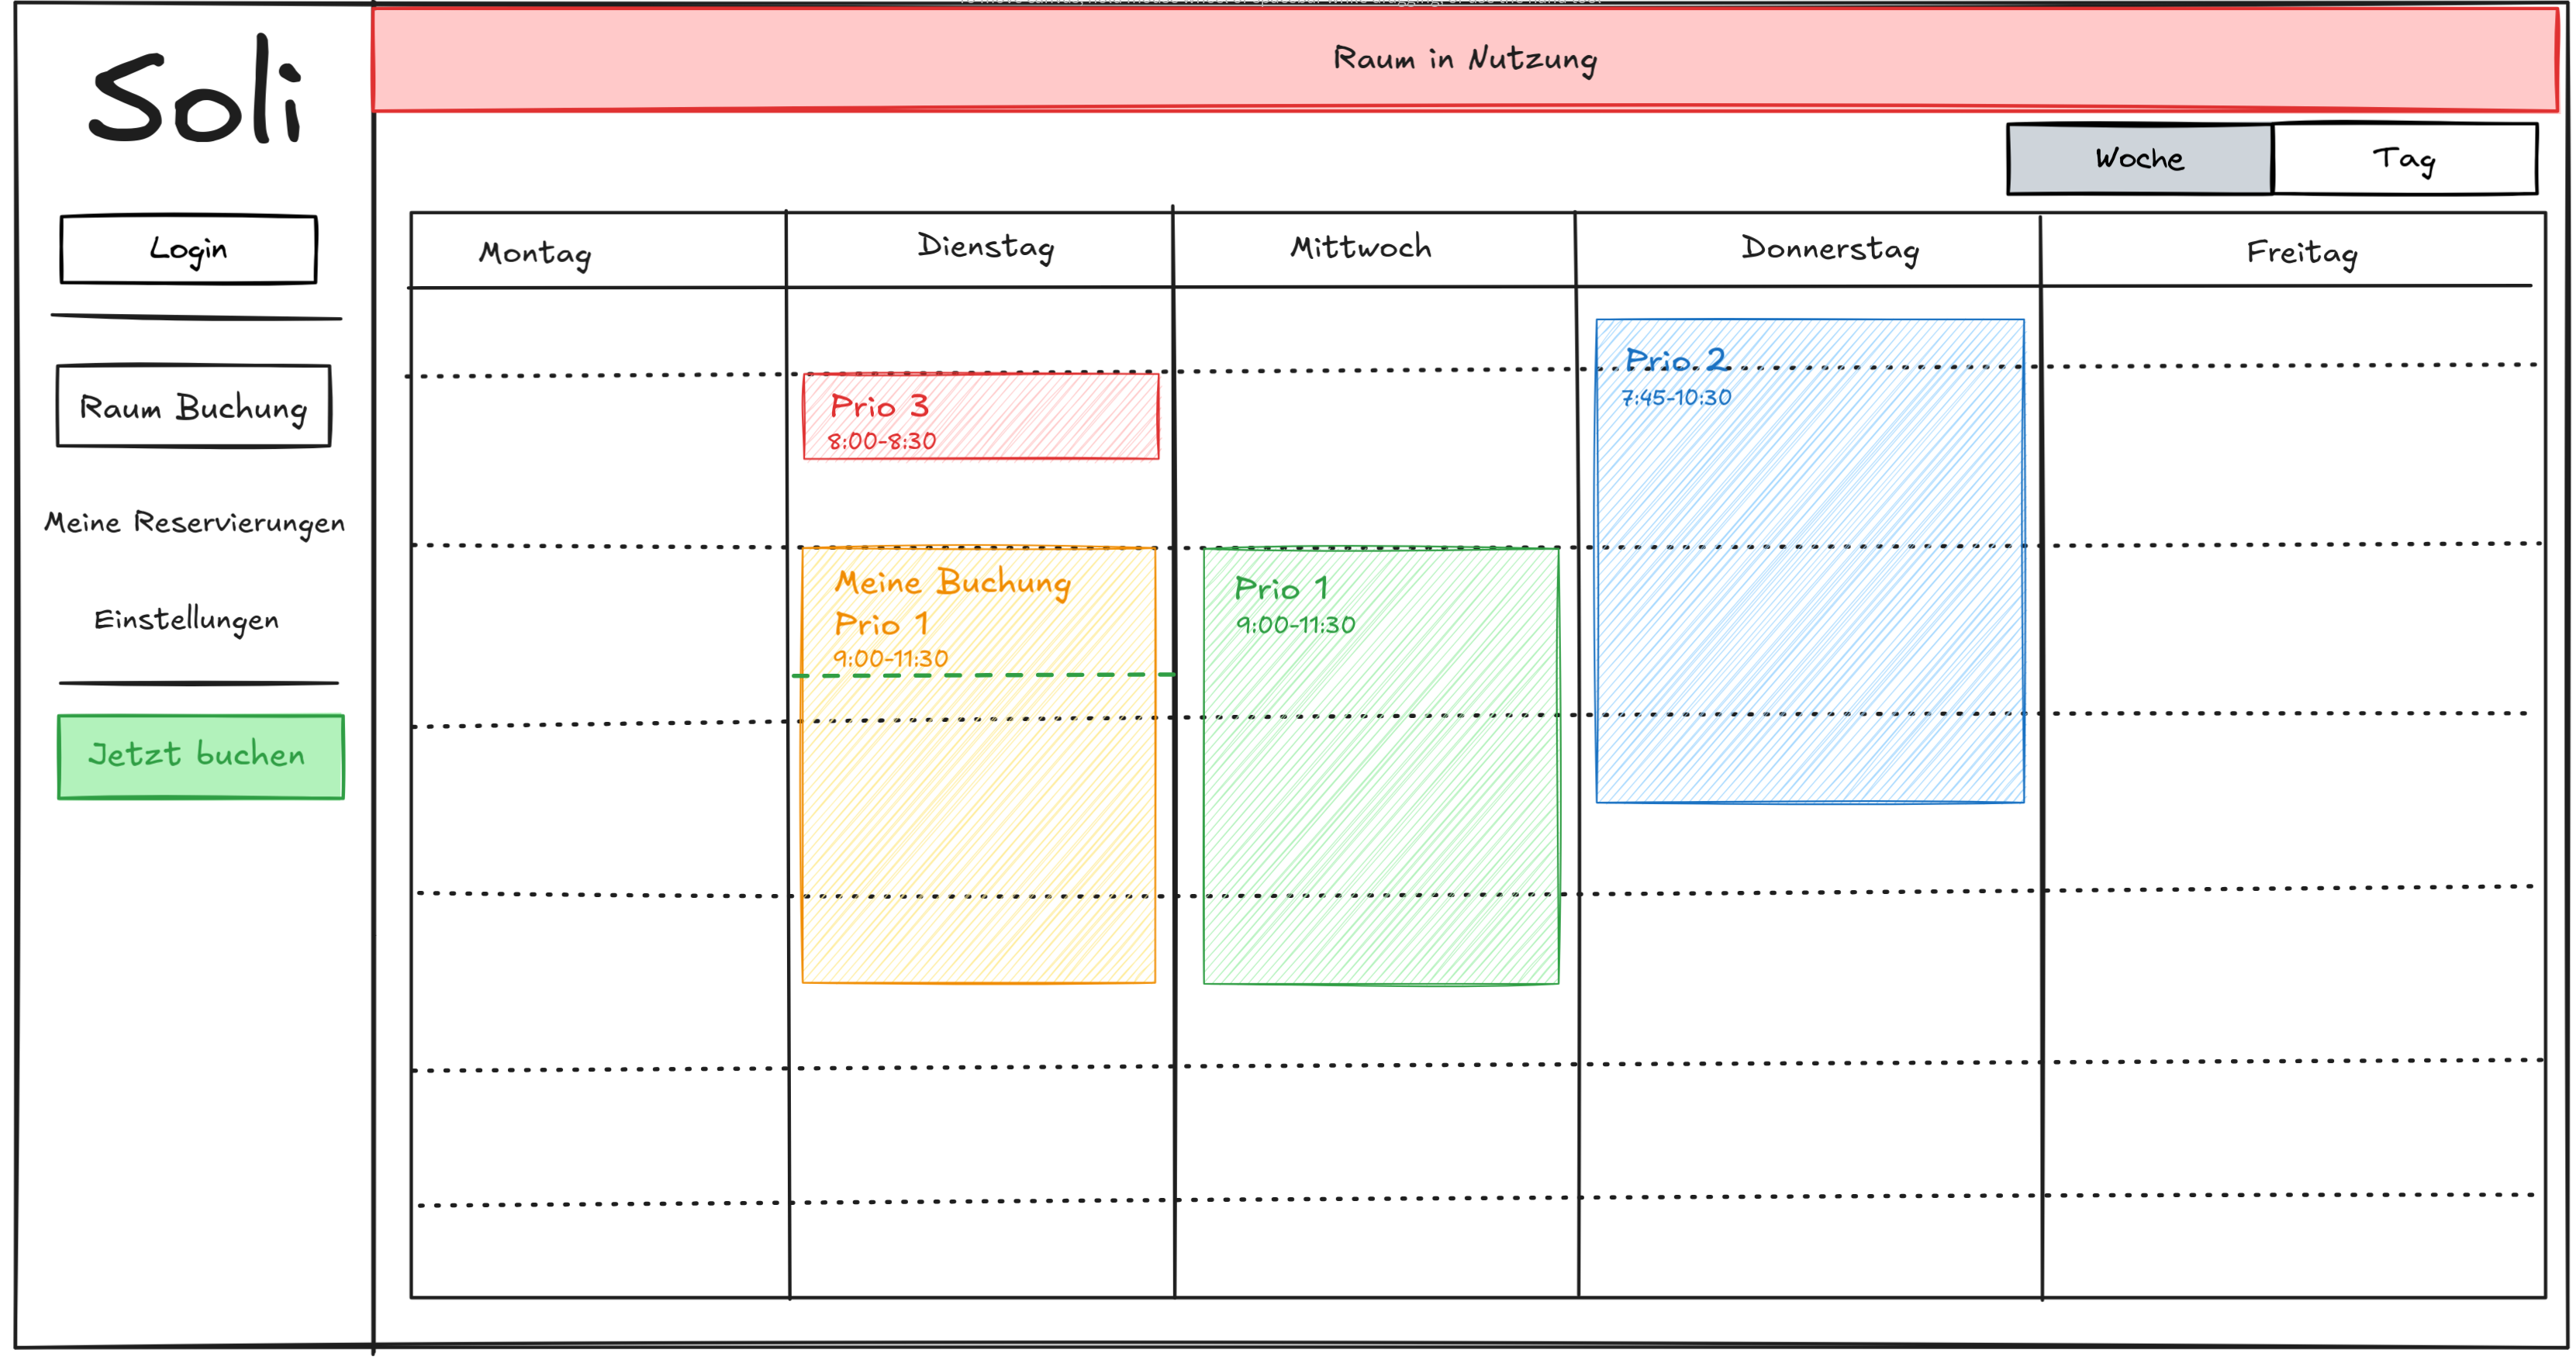
\includegraphics[scale=0.15]{figures/ui/startseite.png}
    \caption{Startseite der Anwendung}
    \label{fig:startseite}
\end{figure}

\begin{figure}[ht]
    \centering
    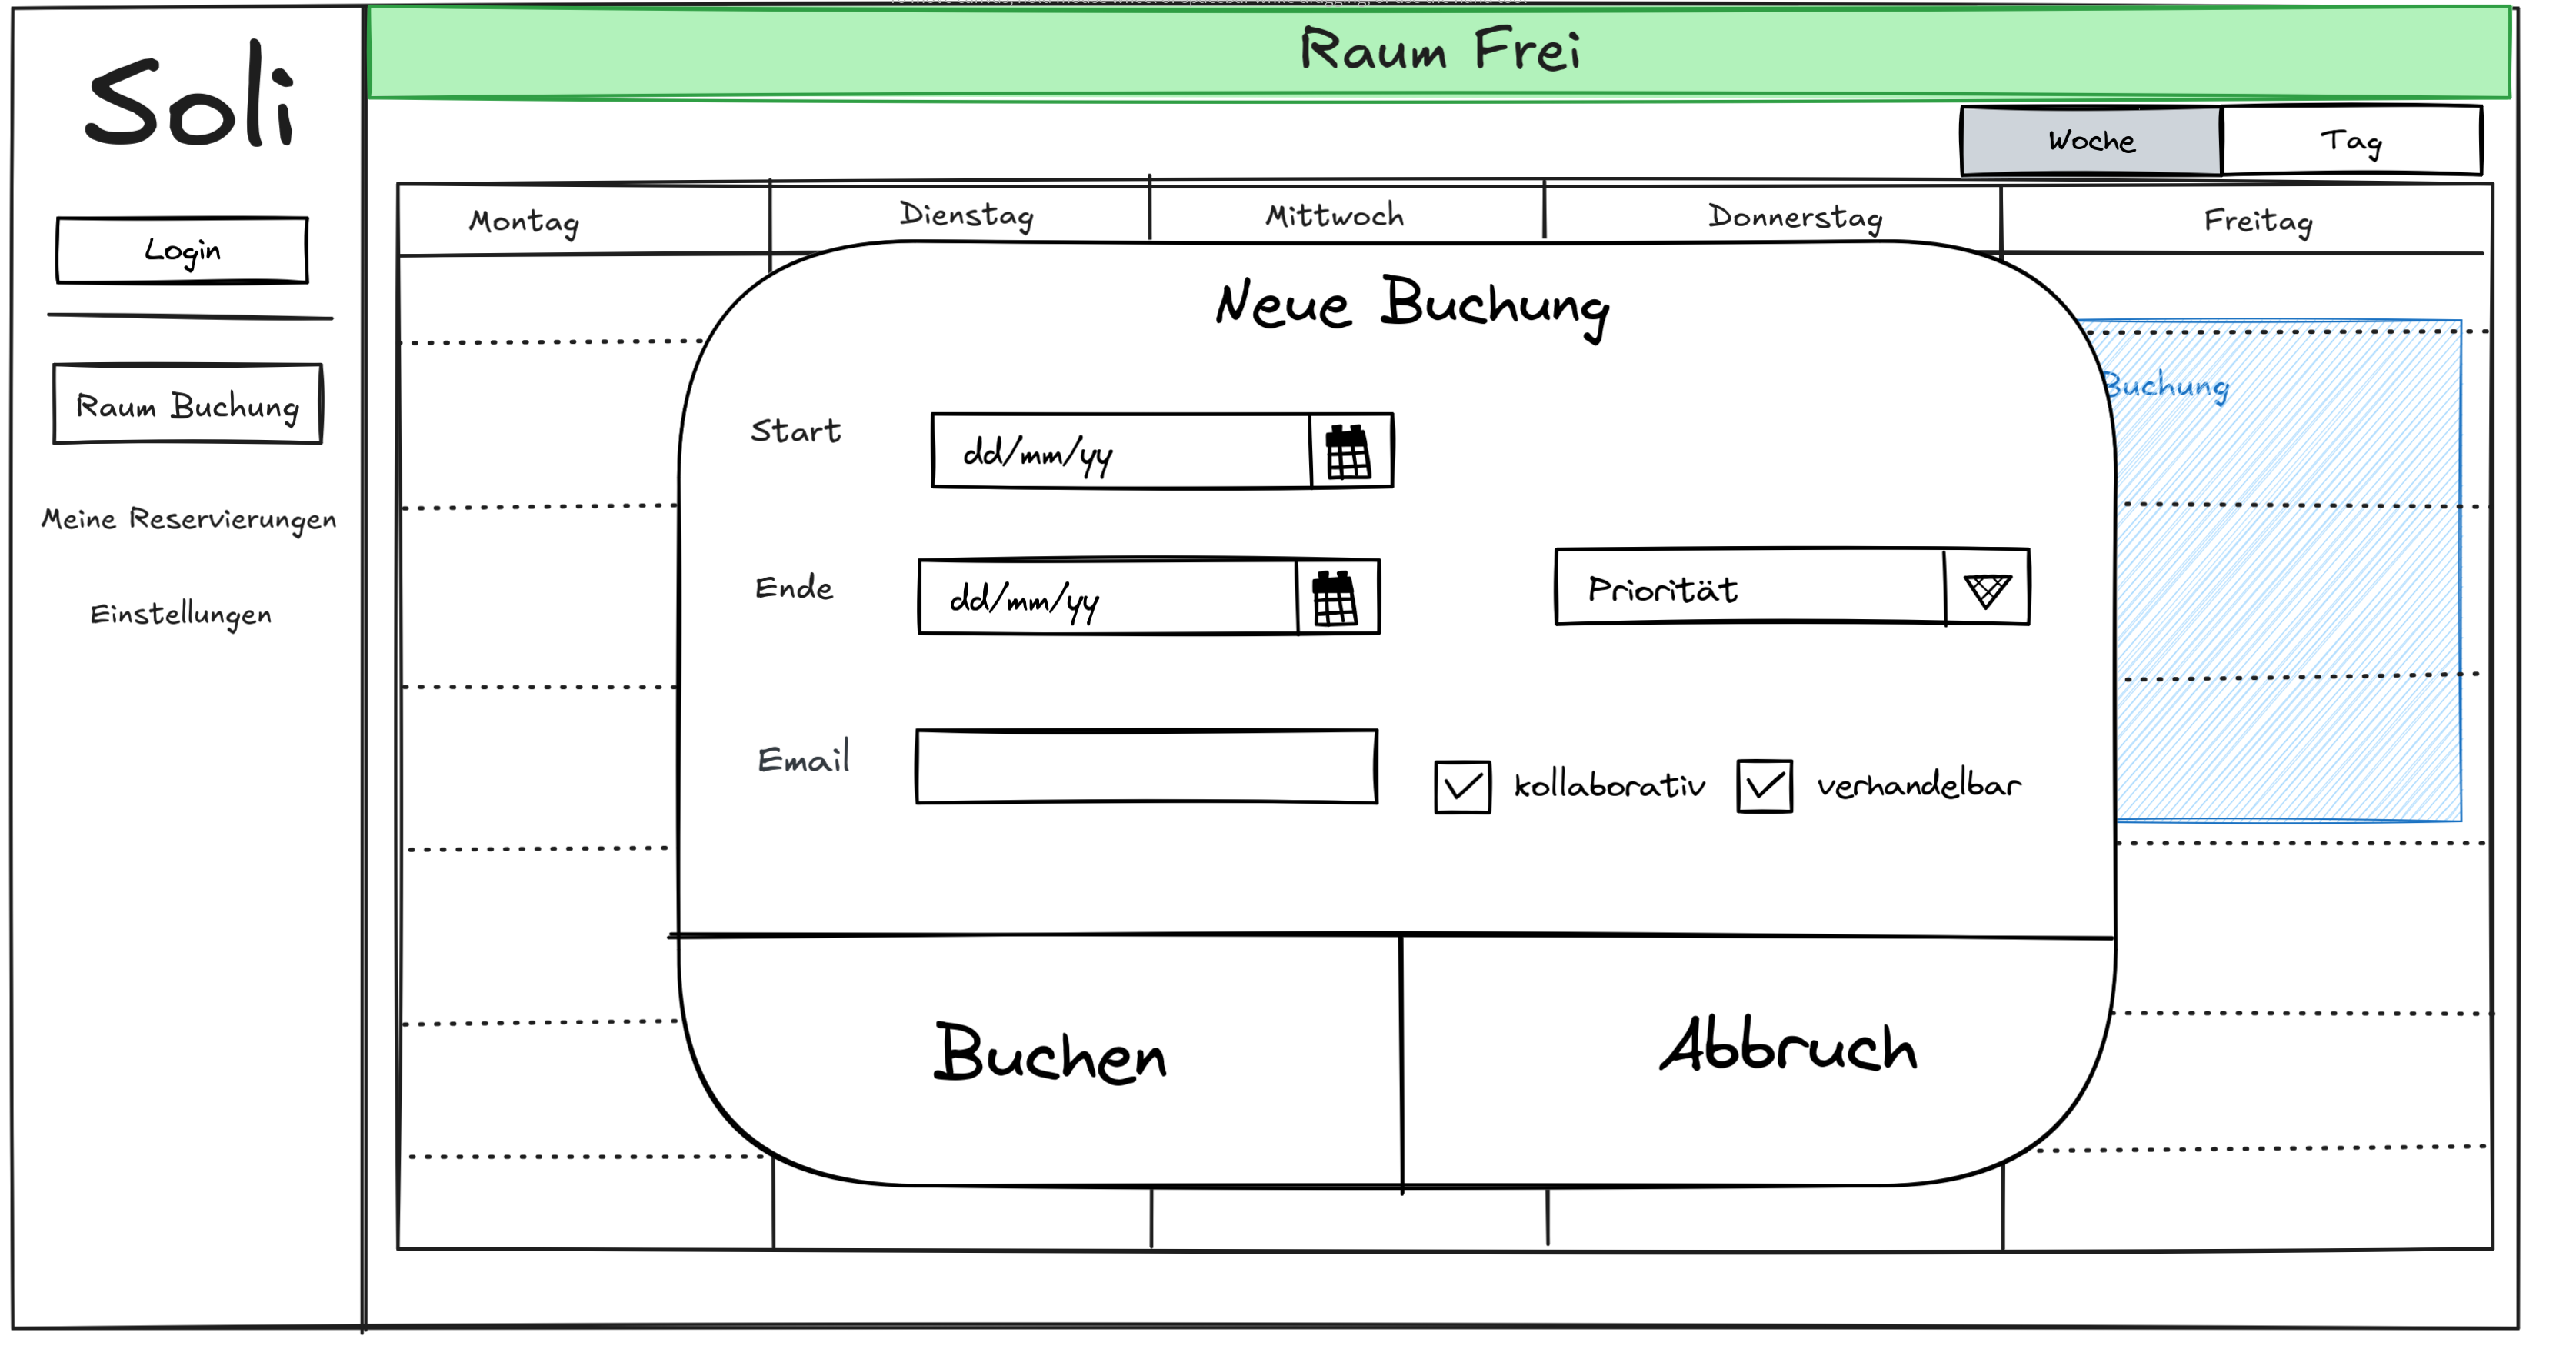
\includegraphics[scale=0.15]{figures/ui/buchungsdialog.png}
    \caption{Buchungsdialog}
    \label{fig:buchung}
\end{figure}

\begin{figure}[ht]
    \centering
    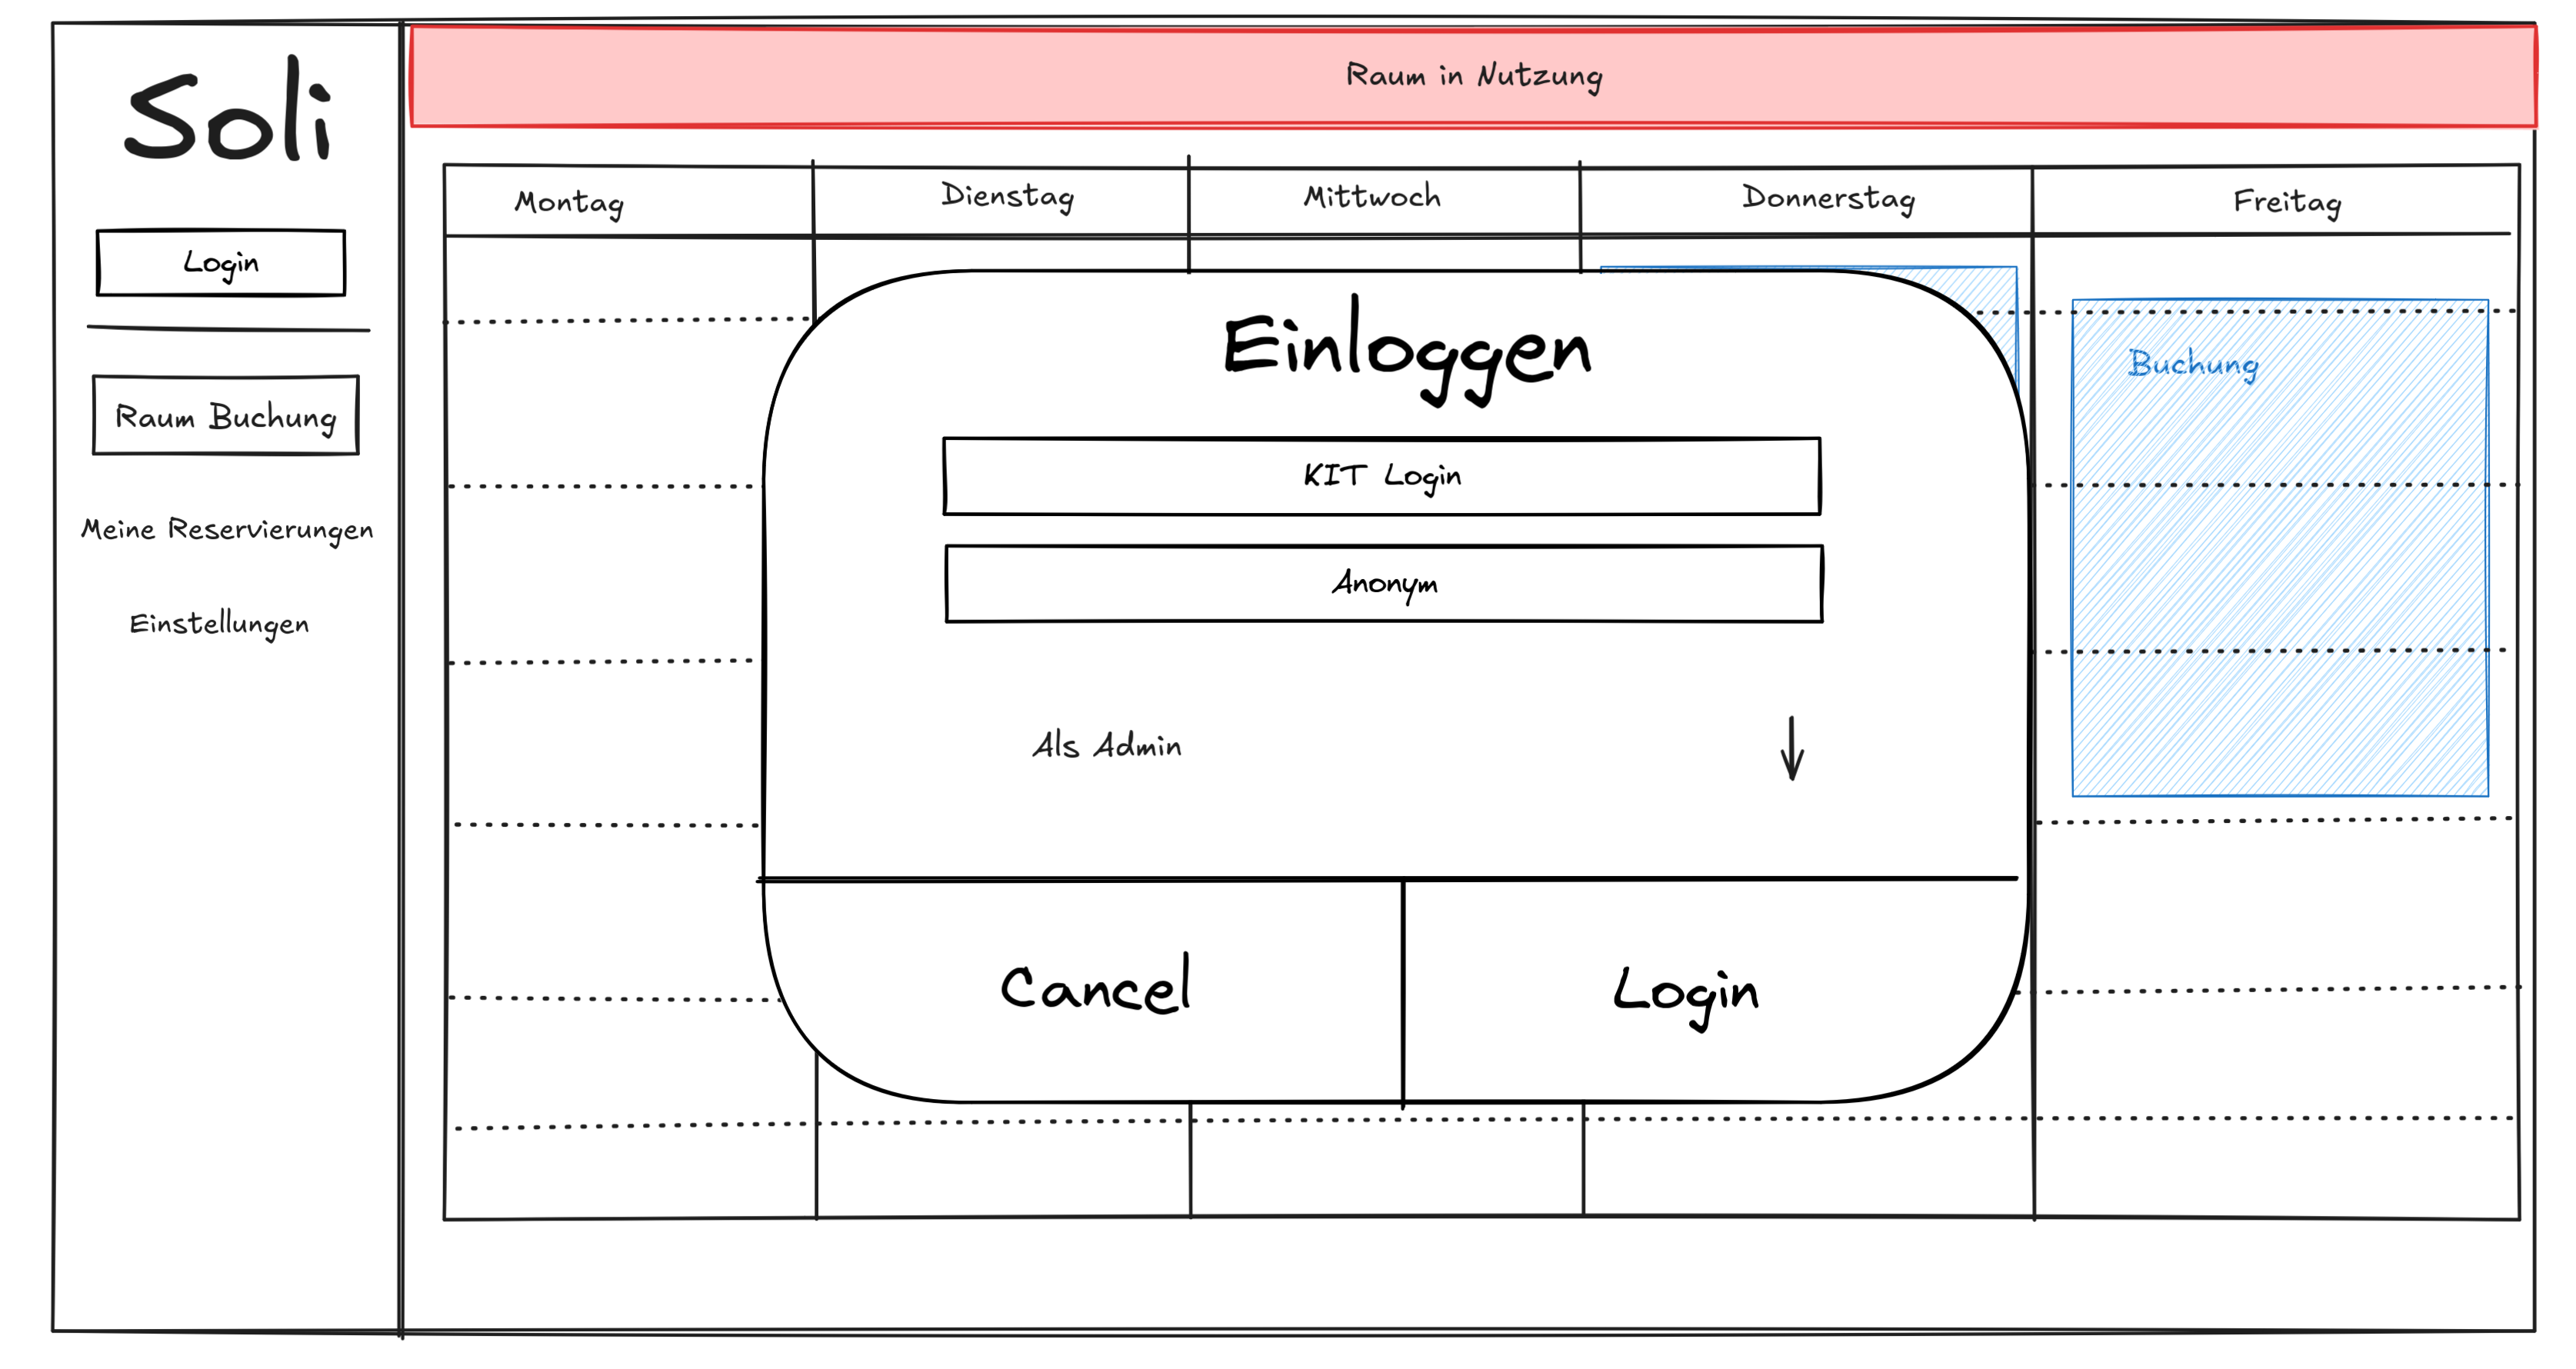
\includegraphics[scale=0.15]{figures/ui/anmeldungsseite.png}
    \caption{Anmeldungsseite}
    \label{fig:login}
\end{figure}

\begin{figure}[ht]
    \centering
    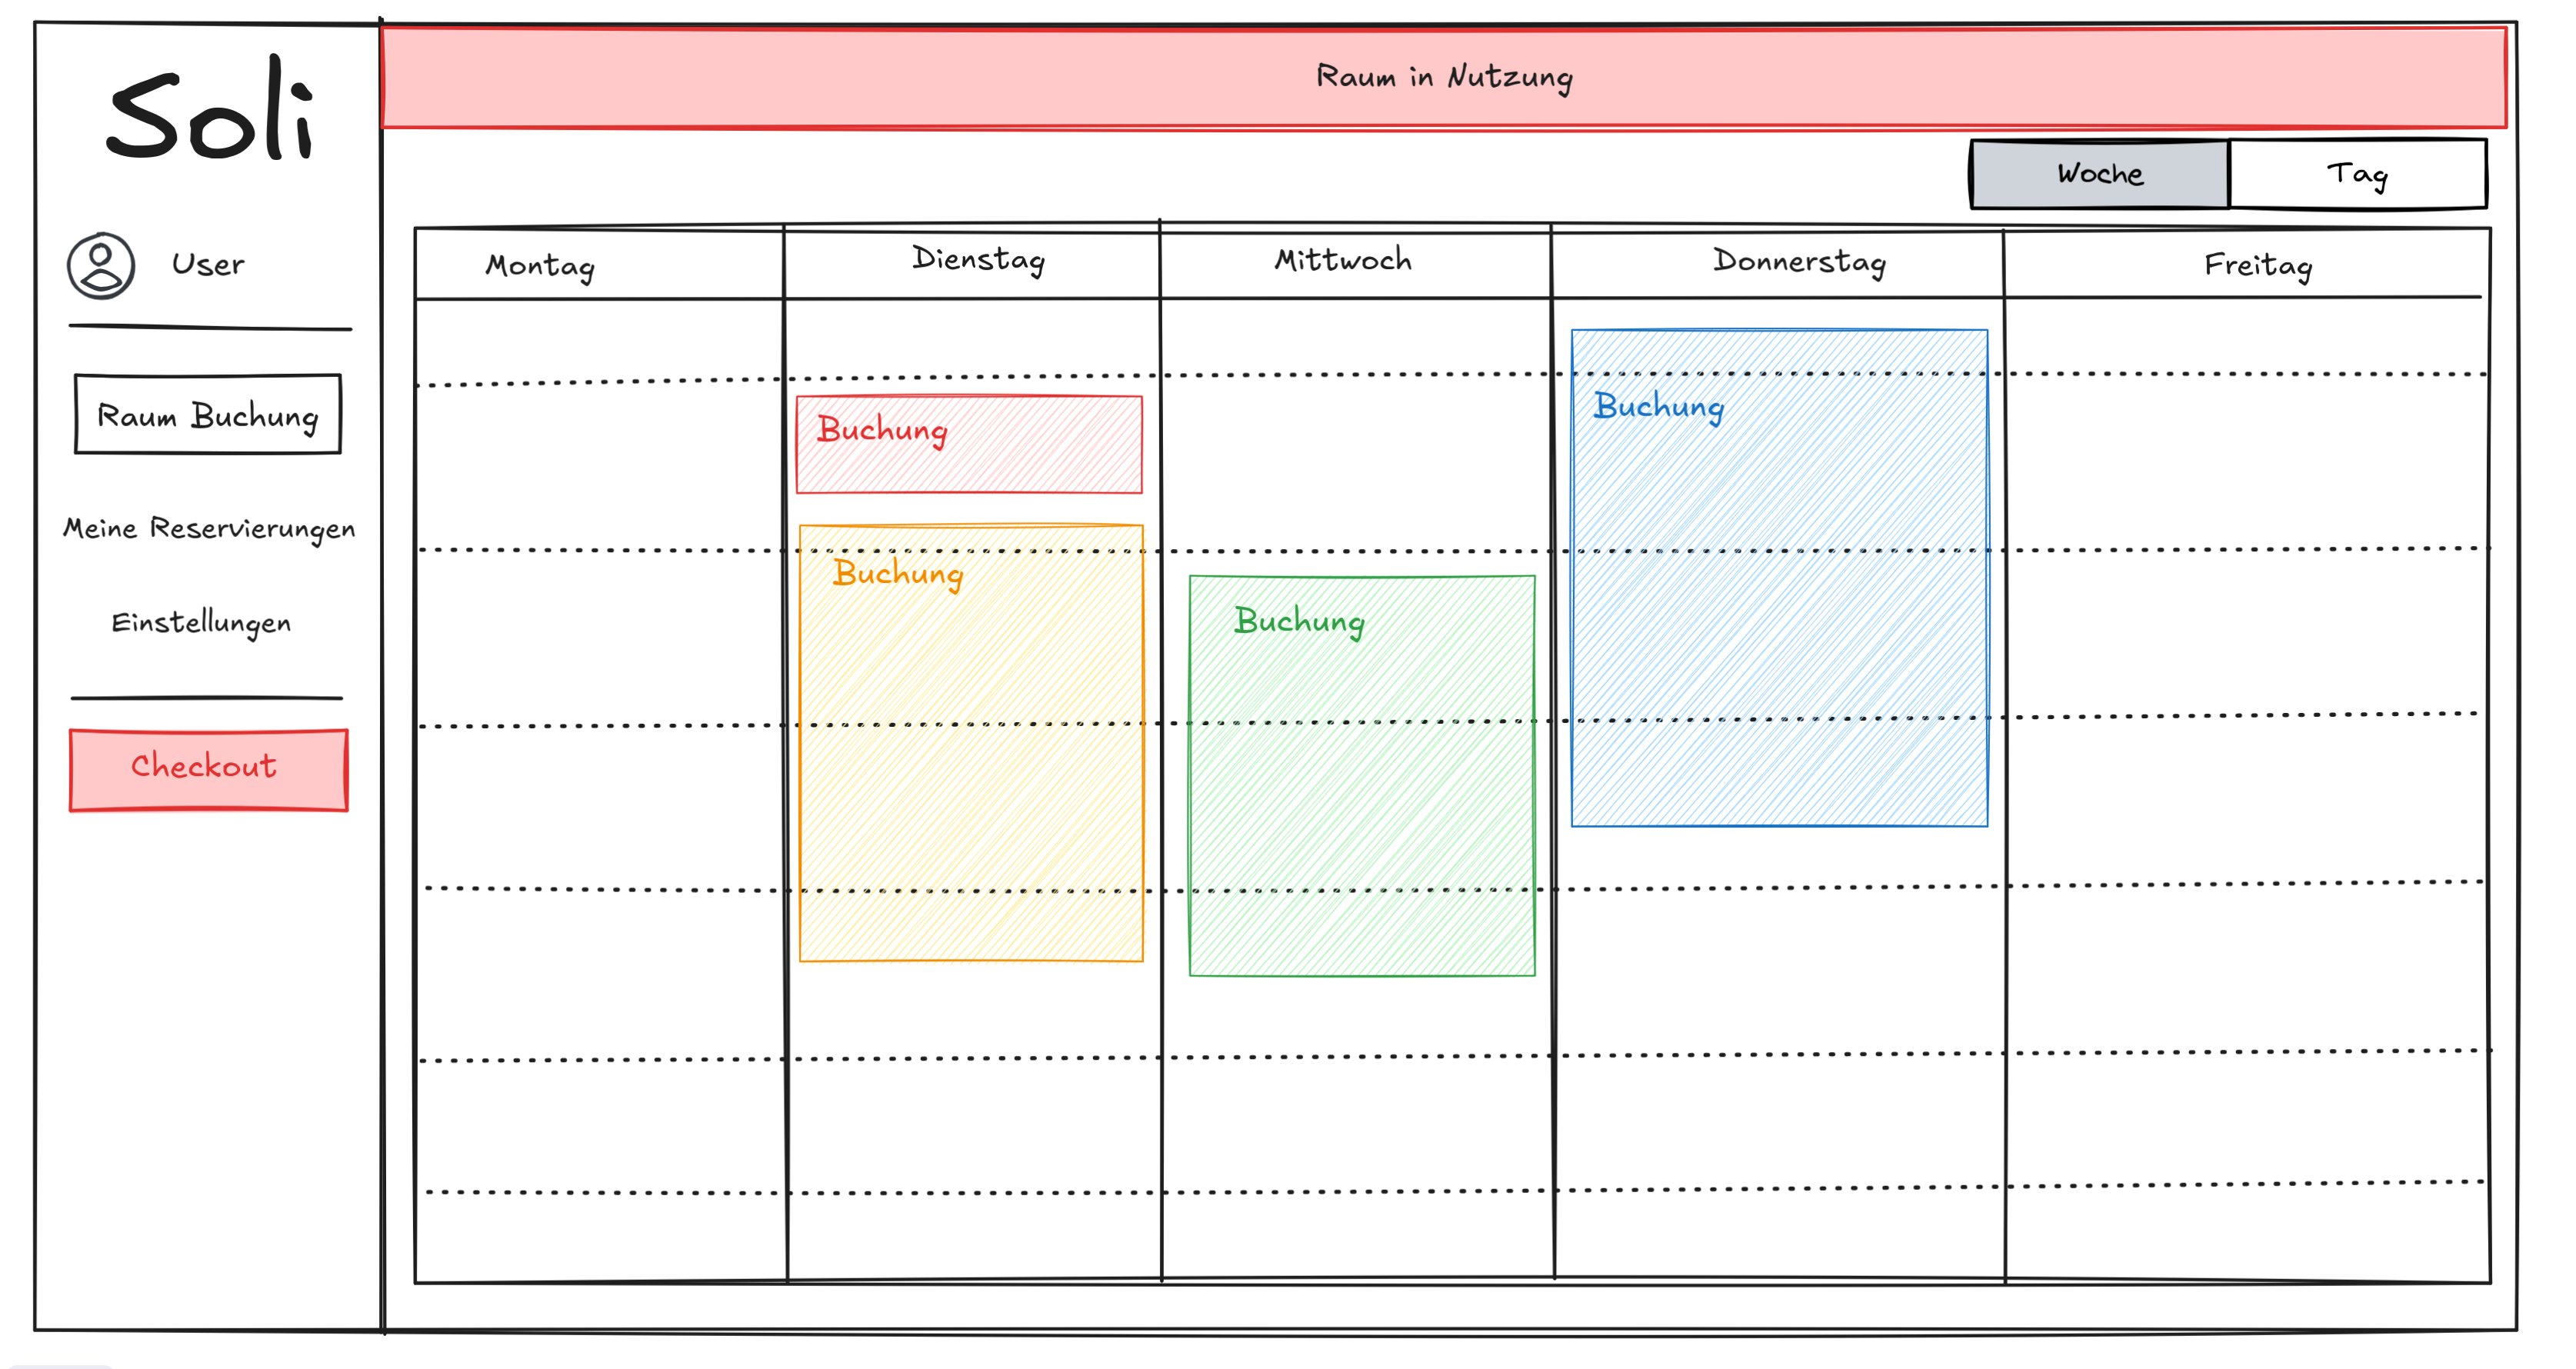
\includegraphics[scale=0.15]{figures/ui/checkout.png}
    \caption{Quick Checkout}
    \label{fig:checkout}
\end{figure}
\clearpage
\section{Buchungsverwaltung}
Sollte ein Benutzer eine Buchung vorgenommen haben, so kann dieser in der Reservierungsübersicht, die in Abbildung \ref{fig:overview} dargestellt ist, seine Buchungen einsehen und verwalten.

\begin{figure}[ht]
    \centering
    \includegraphics[scale=0.15]{figures/ui/reservierungsübersicht.png}
    \caption{Reservierungsübersicht}
    \label{fig:overview}
\end{figure}

\clearpage
\section{Adminstration}
Ein Adminitrator hat die Möglichkeit, über die Benutzeradminstrationsoberfläche, die in Abbildung \ref{fig:adminuser} dargestellt ist, NutzerInnen einzusehen und zu verwalten.
So dient diese Ansicht bspw. dazu NuterInnen zu sperren oder zu entsperren.

\begin{figure}[ht]
    \centering
    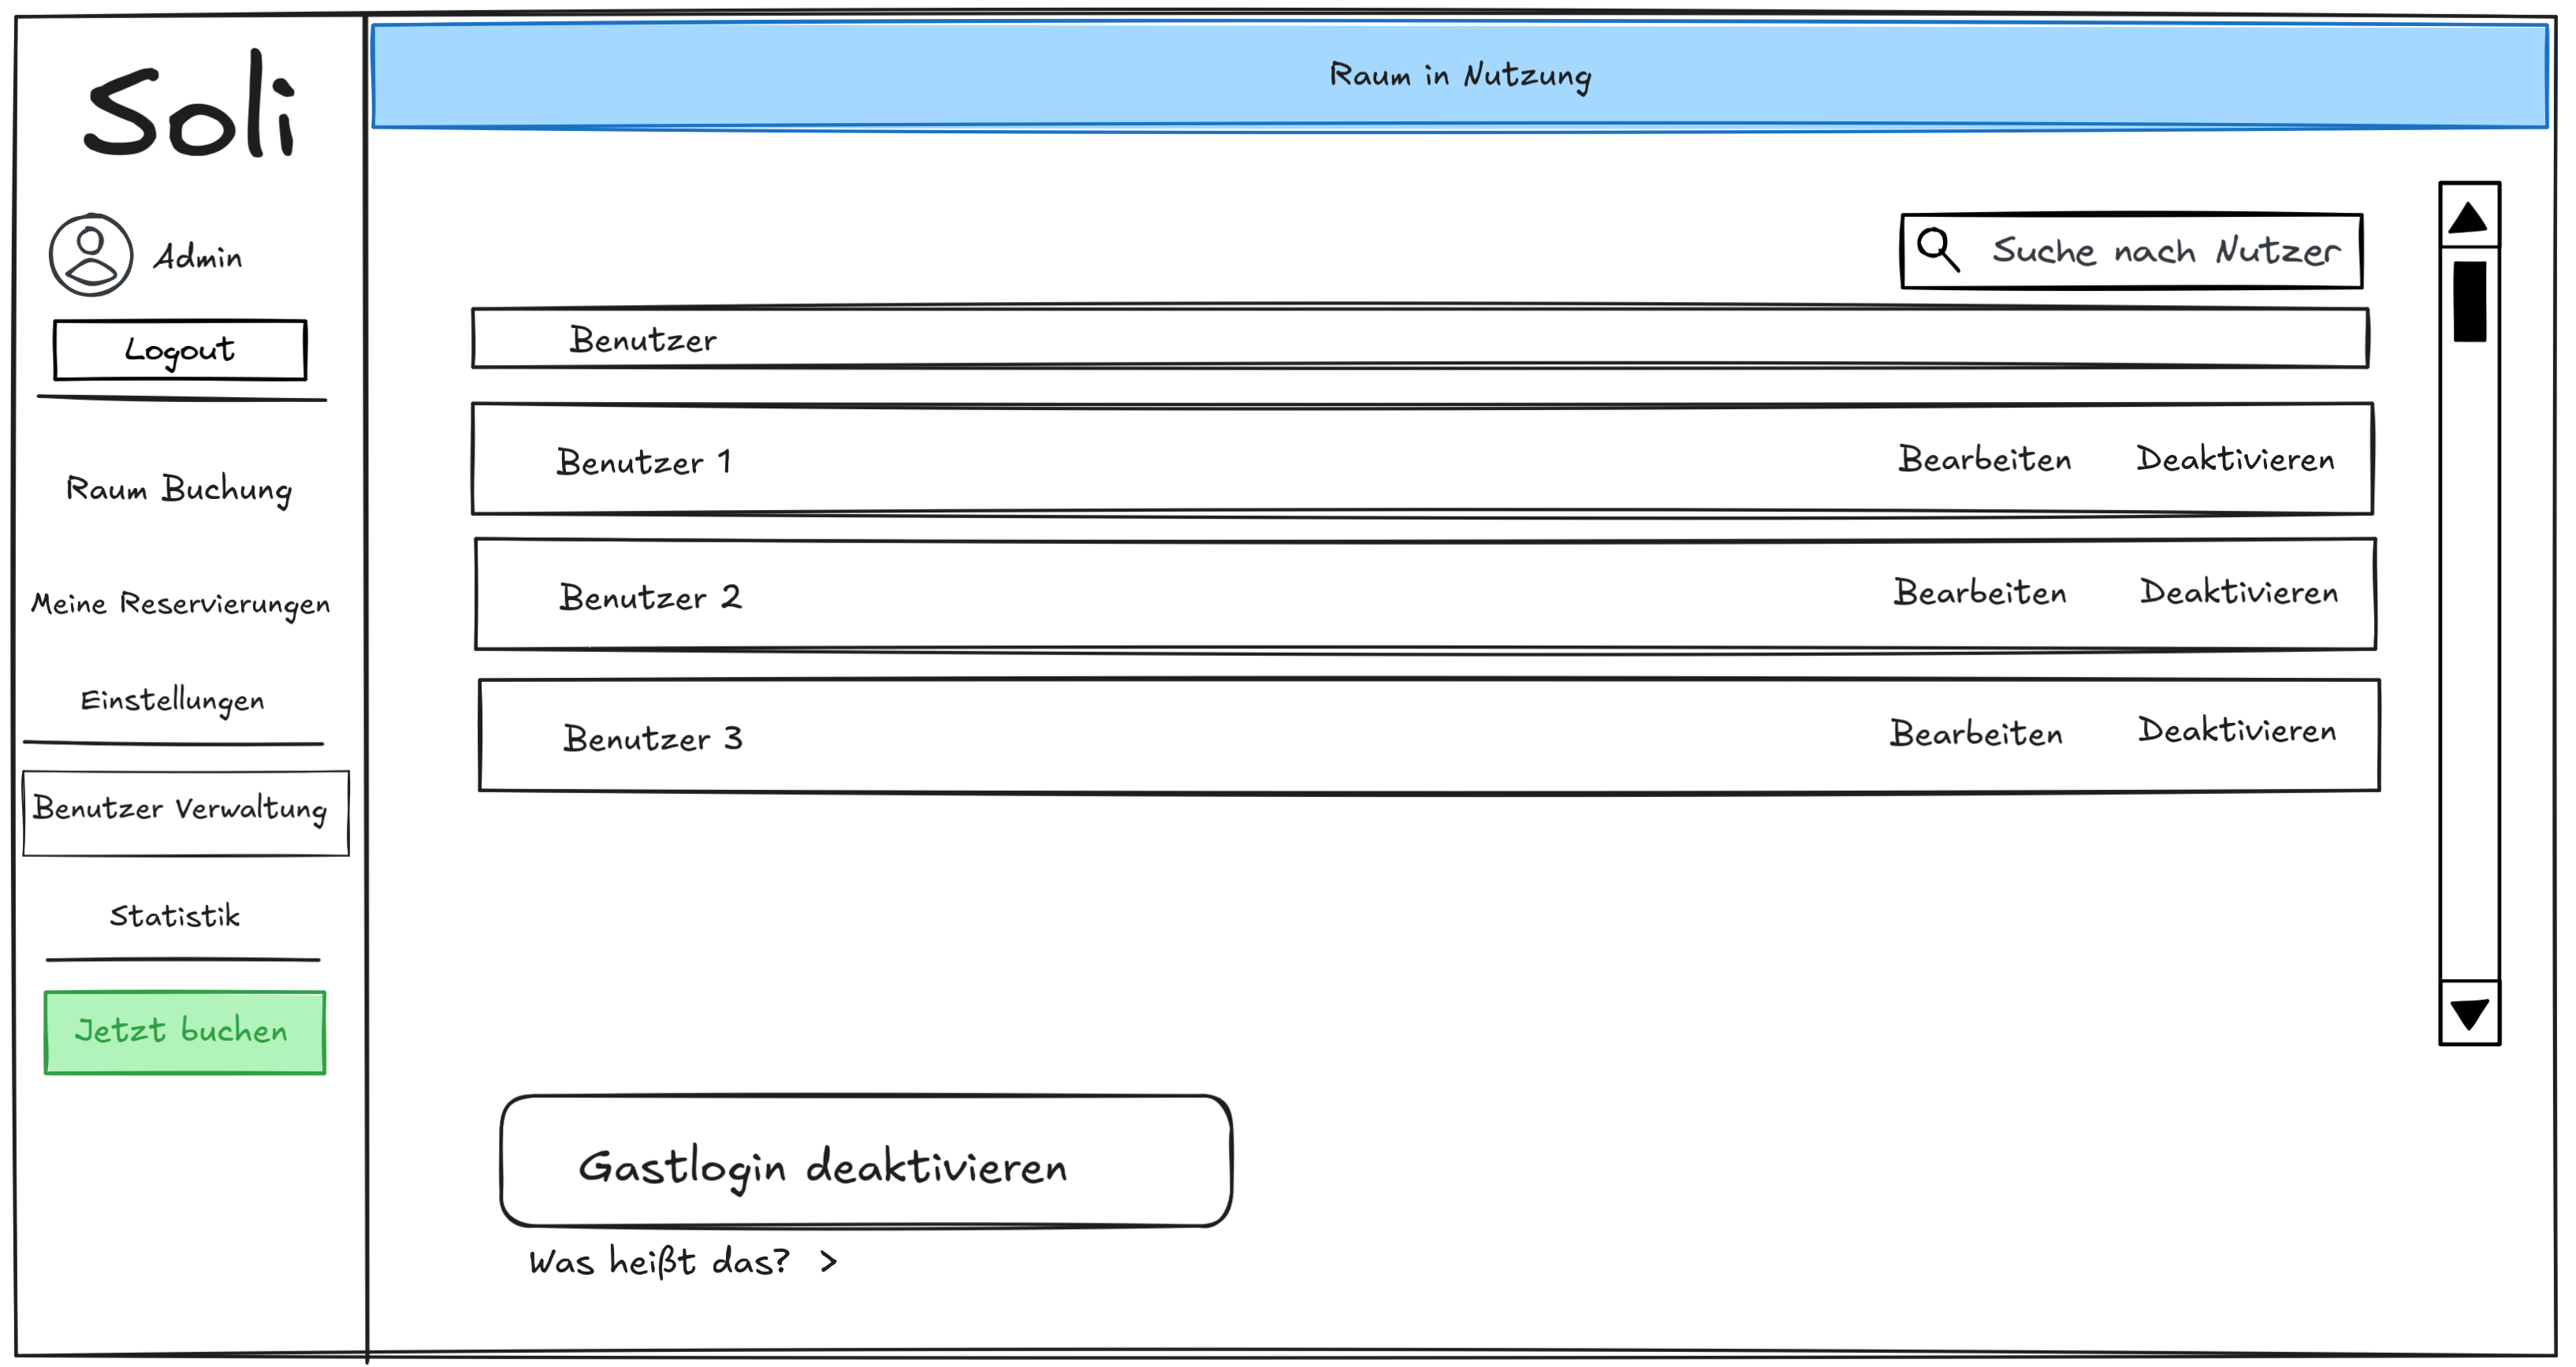
\includegraphics[scale=0.15]{figures/ui/useradminui.png}
    \caption{Benutzeradminstrationsoberfläche}
    \label{fig:adminuser}
\end{figure}

